\section*{Bonus: Topic \& Emotion Analysis (+5 pts)}

\subsection{Topic Modeling}
\textit{Perform a topic modeling using the Latent Dirichlet Allocation (LDA) approach. Explain the foundations of this approach and provide the code snippet used to apply this method. Finally provide a visualization of your results and detail the conclusions you can draw about the COVID-19 epidemics using topic modeling. Compare your results with the Nature article which performs a similar analysis. Hypothesize on why results might be different.}

Latent Dirichlet allocation (LDA) \cite{lda} is a method used to infer topics from text. These topics are not known in advance, and are supposed to be inferred from the words that are grouped under them after training of the model.

\begin{listing*}[t]
\begin{minted}{python}
! pip install pyLDAvis

from gensim.corpora.dictionary import Dictionary
from gensim.models import LdaModel,CoherenceModel
import pyLDAvis
import pyLDAvis.gensim

diction = Dictionary(df_tweets_preprocessed['unigram'])
corpus = [diction.doc2bow(i) for i in df_tweets_preprocessed['unigram']]
n_topics = 4
lda = LdaModel(corpus, id2word=diction, num_topics=n_topics, random_state=42, passes=2)

#inspired by https://www.machinelearningplus.com/nlp/topic-modeling-gensim-python/
# Compute Perplexity
print('\nPerplexity: ', lda.log_perplexity(corpus))  # a measure of how good the model is. lower the better.

# Compute Coherence Score
coherence_model_lda = CoherenceModel(model=lda, texts=df_tweets_preprocessed['unigram'], dictionary=diction, coherence='c_v')
coherence_lda = coherence_model_lda.get_coherence()
print('\nCoherence Score: ', coherence_lda)

pyLDAvis.enable_notebook()
vis = pyLDAvis.gensim.prepare(lda, corpus, diction,R=10)
vis

\end{minted}
\caption{}
\label{listing:pb-code1}
\end{listing*}


We inferred the following topics from LDA: covid safety rules (containing words such as: 'stay' and 'home', 'social' and 'distancing', 'mask'), government and politics (containing words like: 'Trump', 'lockdown', 'president', and 'pm' ), news reports (containing words like 'new' and 'cases', 'pandemic', 'death', 'China'), and a covid-related topic we could not find a common term for (containing words such as 'quarantine', 'know', 'like', 'thing', 'lockdown', 'day', and 'one'). The histogram of the topic frequencies can be found in Figure \ref{fig:lda_histo}, and the words related to each topic can be found in Figure \ref{fig:lda_viz}

\begin{figure}
 \centering
 \begin{subfigure}{0.5\columnwidth}
 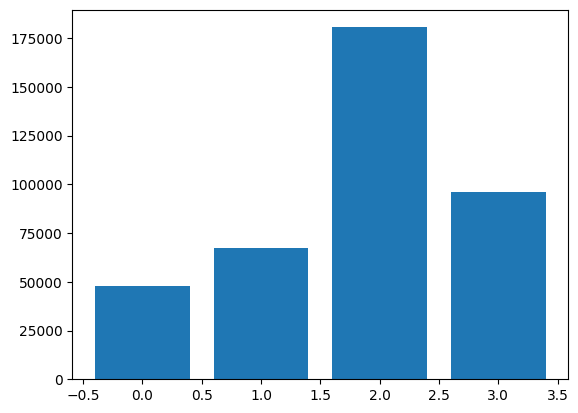
\includegraphics[width=1\textwidth]{images/LDA_topics.png}
 \end{subfigure}
 \caption{Most common topics in the TweetsCov19 dataset. Topic 1 corresponds to the unknown topic, topic 2 to 'news reports', topic 3 to 'covid safety rules', and topic 4 to 'government and politics'.}
 \label{fig:lda_histo}
\end{figure}


Different from the Nature article \cite{ldaUK}, we were unable to find more than 4 sensible topics, with topics beyond 3 often strongly overlapping with one another. This is likely due to the fact that we are using a different dataset and different preprocessing methods. Their dataset is almost double the size (800 000 tweets), and contains tweets from the UK only, while ours contains tweets from across the world (the majority from the US, which is probably a big reason why Trump is so prominent in one of the topics)


\begin{figure}
 \centering
 \begin{subfigure}{0.75\columnwidth}
 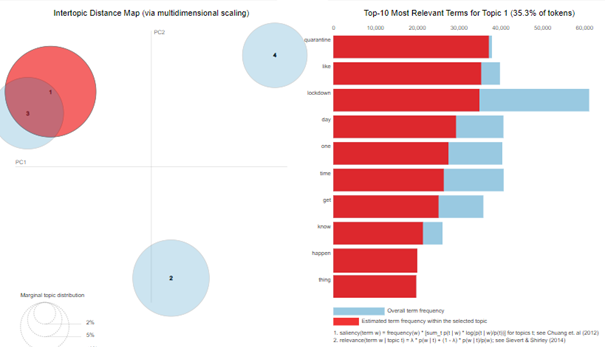
\includegraphics[width=1\textwidth]{images/lda1.png}
 \end{subfigure}
 \centering
 \begin{subfigure}{0.75\columnwidth}
 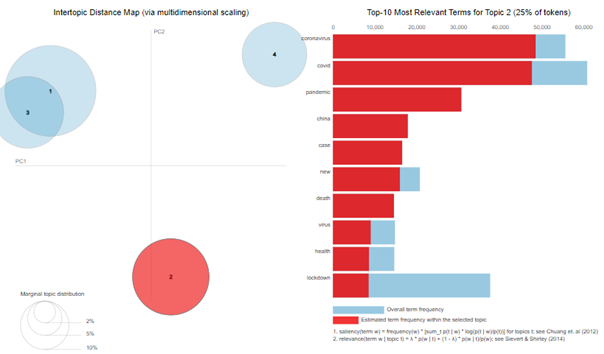
\includegraphics[width=1\textwidth]{images/lda2.png}
 \end{subfigure}
 \caption{Visualization of the topics inferred from LDA. Topic 1 corresponds to the unknown topic and topic 2 to 'news reports'.}
 \label{fig:lda_viz}
\end{figure}



\begin{figure}
 \ContinuedFloat
 \centering
 \begin{subfigure}{0.75\columnwidth}
 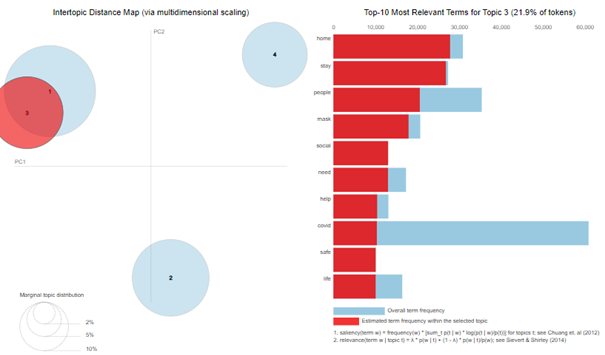
\includegraphics[width=1\textwidth]{images/lda3.png}
 \end{subfigure}
 \centering
 \begin{subfigure}{0.75\columnwidth}
 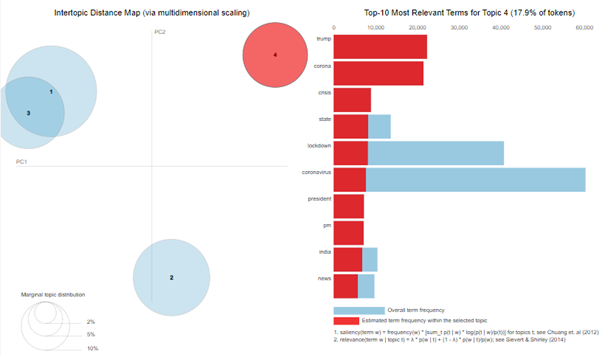
\includegraphics[width=1\textwidth]{images/lda4.png}
 \end{subfigure}
 \caption{(continued) Visualization of the topics inferred from LDA. Topic 3 corresponds to 'covid safety rules', and topic 4 to 'government and politics'.}
 \label{fig:lda_viz}
\end{figure}


